\chapter{Dashboardvisualisierung} % 5-6 Seiten? 
\label{ch:auswahl}
Im vorherigen Kapitel wurde beschrieben, wie Nutzerdaten erfasst werden können. Hierfür wurden relevante KPIs für das Bildungsportal definiert und verschiedene Methoden der Datenerhebung sowie deren DSGVO-konforme Umsetzung beschrieben. Um die gesammelten Daten strukturiert und übersichtlich darzustellen und der Professur für Geschichtsdidaktik eine fundierte Grundlage für datenbasierte Erkenntnisse zu bieten, sollen die KPIs visuell auf einem Dashboard aufbereitet werden. Dazu werden zunächst die eigenen Anforderungen an das Dashboard erörtert. Anschließend werden geeignete Visualisierungsmethoden für die KPIs vorgestellt und die Struktur sowie der Aufbau des Dashboards festgelegt. Abschließend wird Grafana als Visualisierungslösung evaluiert. Hierbei wird auf das Kapitel~\ref{sec:anforderungen} Bezug genommen und beschrieben wie selbst definierten technisch-funktionalen-,sowie Usability- und Design Anforderungen in Grafana realisiert werden können. 

\section{Anforderungen an das Dashboard}
\label{sec:anforderungen}
\subsection{Technisch-funktionale Anforderungen}
Die technisch-funktionalen Anforderungen sollen bei der Auswahl einer Dashboard Lösung Orientierung geben. Welche Funktionen ein Dashboard bereitstellen muss und welche technologischen Rahmenbedingungen erfüllt sein sollten, um eine effiziente und stabile Nutzung zu gewährleisten. Diese Anforderungen sind: 
\begin{itemize}
    \item \textbf{Datenintegration und Aggregation:} Das Dashboard Tool soll in der Lage sein, Daten aus Matomo oder alternativ direkt aus der Datenbank zu beziehen und zu aggregieren. Außerdem sollen die per Webanalysetool erfassten Daten automatisch aktualisiert werden. Entweder in definierten Intervallen oder in Echtzeit.
    \item \textbf{Interaktive Funktionen:} Es soll die Möglichkeit geboten werden, die Daten nach einem Datum, Zeitraum und Benutzergruppen zu filtern. (evtl. weitere)
    \item \textbf{Skalierbarkeit und Performance:} Um die Ladezeit des Dashboards zu optimieren, muss es möglich sein Datenabfragen zu optimieren. Um eine bessere Performance zu erreichen sollen die Elemente des Dashboards nach bedarf geladen werden und nicht gleichzeitig. Ebenfalls ist es wichtig, dass das Dashboard bei größer werdenden Datenmengen weiterhin effizient arbeitet.
    \item \textbf{Sicherheit und Zugriffskontrolle:} Um sicherzustellen, dass nur authentifzierte Benutzer zugriff auf das Dashboard haben, muss es eine Anmeldefunktion geben. Ebenfalls soll das Tool über eine HTTPS-Verbindung laufen. API- und Datenquellen- Zugriffe müssen gesichert werden, um unbefugten Zugriff zu verhindern. Ebenfalls soll eine Rollenbasierte Zugriffskontrolle (engl Roll based Access Controll (RBAC)) implementiert werden.
\end{itemize}

\subsection{Usability- und Design Anforderungen}
Neben technischen Aspekten ist die Benutzerfreundlichkeit des Dashboards nicht zu vernachlässigen. Gerade weil das Dashboard in erster Linie von Nicht-Informatikern verwendet wird, ist eine intuitive Gestaltung wichtig, um einen guten Überblick und eine schnelle Orientierung zu ermöglichen. Wichtige Anforderungen sind hierbei: 
\begin{itemize}
    \item \textbf{Anordnung der Inhalte:} Die KPIs sollten so dargestellt werden, dass verwandte Indikatoren auch im Dashboard nebeneinander zu finden sind.
    \item \textbf{Konsistenz in Farben \& Darstellungen:} Ein einheitliches Farbschema soll die Orientierung erleichtern und dient positive (z.B. in grün) und negative (z.B. in rot) Trends einer KPI auf dem ersten Blick zu erkennen. Ebenfalls sollen konsistente Darstellungen für identische KPIs verwendet werden.
    \item \textbf{Interaktive Elemente:} Für KPIs, für welche es sinnvoll ist, sollte das Dashboard eine Drill-Down-Funktion bieten, um detailliertere Analysen zu ermöglichen.
\end{itemize}

\section{Struktur und Aufbau des Dashboards}
Bei der Gestaltung eines Dashboards ist es sinnvoll, inhaltlich zusammenhängende KPIs zu gruppieren, um eine klare Struktur und eine bessere Übersichtlichkeit zu gewährleisten. Besonders bei einer großen Anzahl an Kennzahlen hilft diese Form der Gruppierung dabei, die relevanten Informationen gezielt darzustellen, ohne den Gesamtüberblick zu verlieren. [vlg. Hassler, 2019, Kap. 14.3]

Laut Stephen Few kann die Möglichkeit zur Navigation zwischen unterschiedlichen Ansichten eine sinnvolle Funktion sein, doch sie sollte nur dort eingesetzt werden, wo sie zur Strukturierung beiträgt. Andernfalls kann eine zu starke Fragmentierung die Effizienz eines Dashboards erheblich einschränken, da zusammengehörige Informationen nicht mehr in einem sinnvollen Kontext betrachtet werden können. [Few, 2006, Kap. 3.1.1]

Auch die Notwendigkeit, innerhalb eines Dashboards vertikal oder horizontal zu scrollen, kann die Übersichtlichkeit beeinträchtigen. Laut Few führt dies dazu, dass Nutzer nicht auf einen Blick alle wichtigen Daten erfassen können und häufig nicht bemerken, dass sich weitere relevante Informationen außerhalb ihres sichtbaren Bereichs befinden. Elemente, die nicht sofort sichtbar sind, werden oft als weniger wichtig wahrgenommen oder gar übersehen, was die Effektivität eines Dashboards erheblich einschränken kann. [Few, 2006, Kap. 3.1.1]

Für das Bildungsportal evaschiffmann.de ist es daher sinnvoll, die KPIs auf dedizierten Dashboard-Seiten darzustellen, da diese jeweils demselben Kontext dienen und somit das scrollen vermieden werden kann, welches ohne eine solche Aufteilung auf Grund der Menge unumgänglich wäre. Die KPIs wurden in Kapitel~\ref{sec:kpis} bereits entsprechend für die einzelnen Webseiten des Bildungsportals definiert. Diese Struktur ermöglicht eine gezielte Analyse der verschiedenen Bereiche, weshalb das Dashboard ebenso aufgebaut wird.

\subsection{Anordnung der Elemente}
Um nun die einzelnen KPIs der jeweiligen Dashboardseiten so anzuordnen, dass Indikatoren, welche dem selben Kontext dienen nah bei einander angezeigt werden, empfiehlt sich eine Gruppierung nach Untersuchungsthema [vlg. Hassler, 2019, Kap. 14.3]. Um eine solche Gruppierung zu realisieren, ist es sinnvoll das Dashboard in Dimensionen einzuteilen und die einzelnen KPIs an eine Dimension zu binden. Hierzu gibt folgendes Modell in Abbildung ~\ref{fig:dimensionen} auskunft: 

\begin{figure}[h]
    \centering
    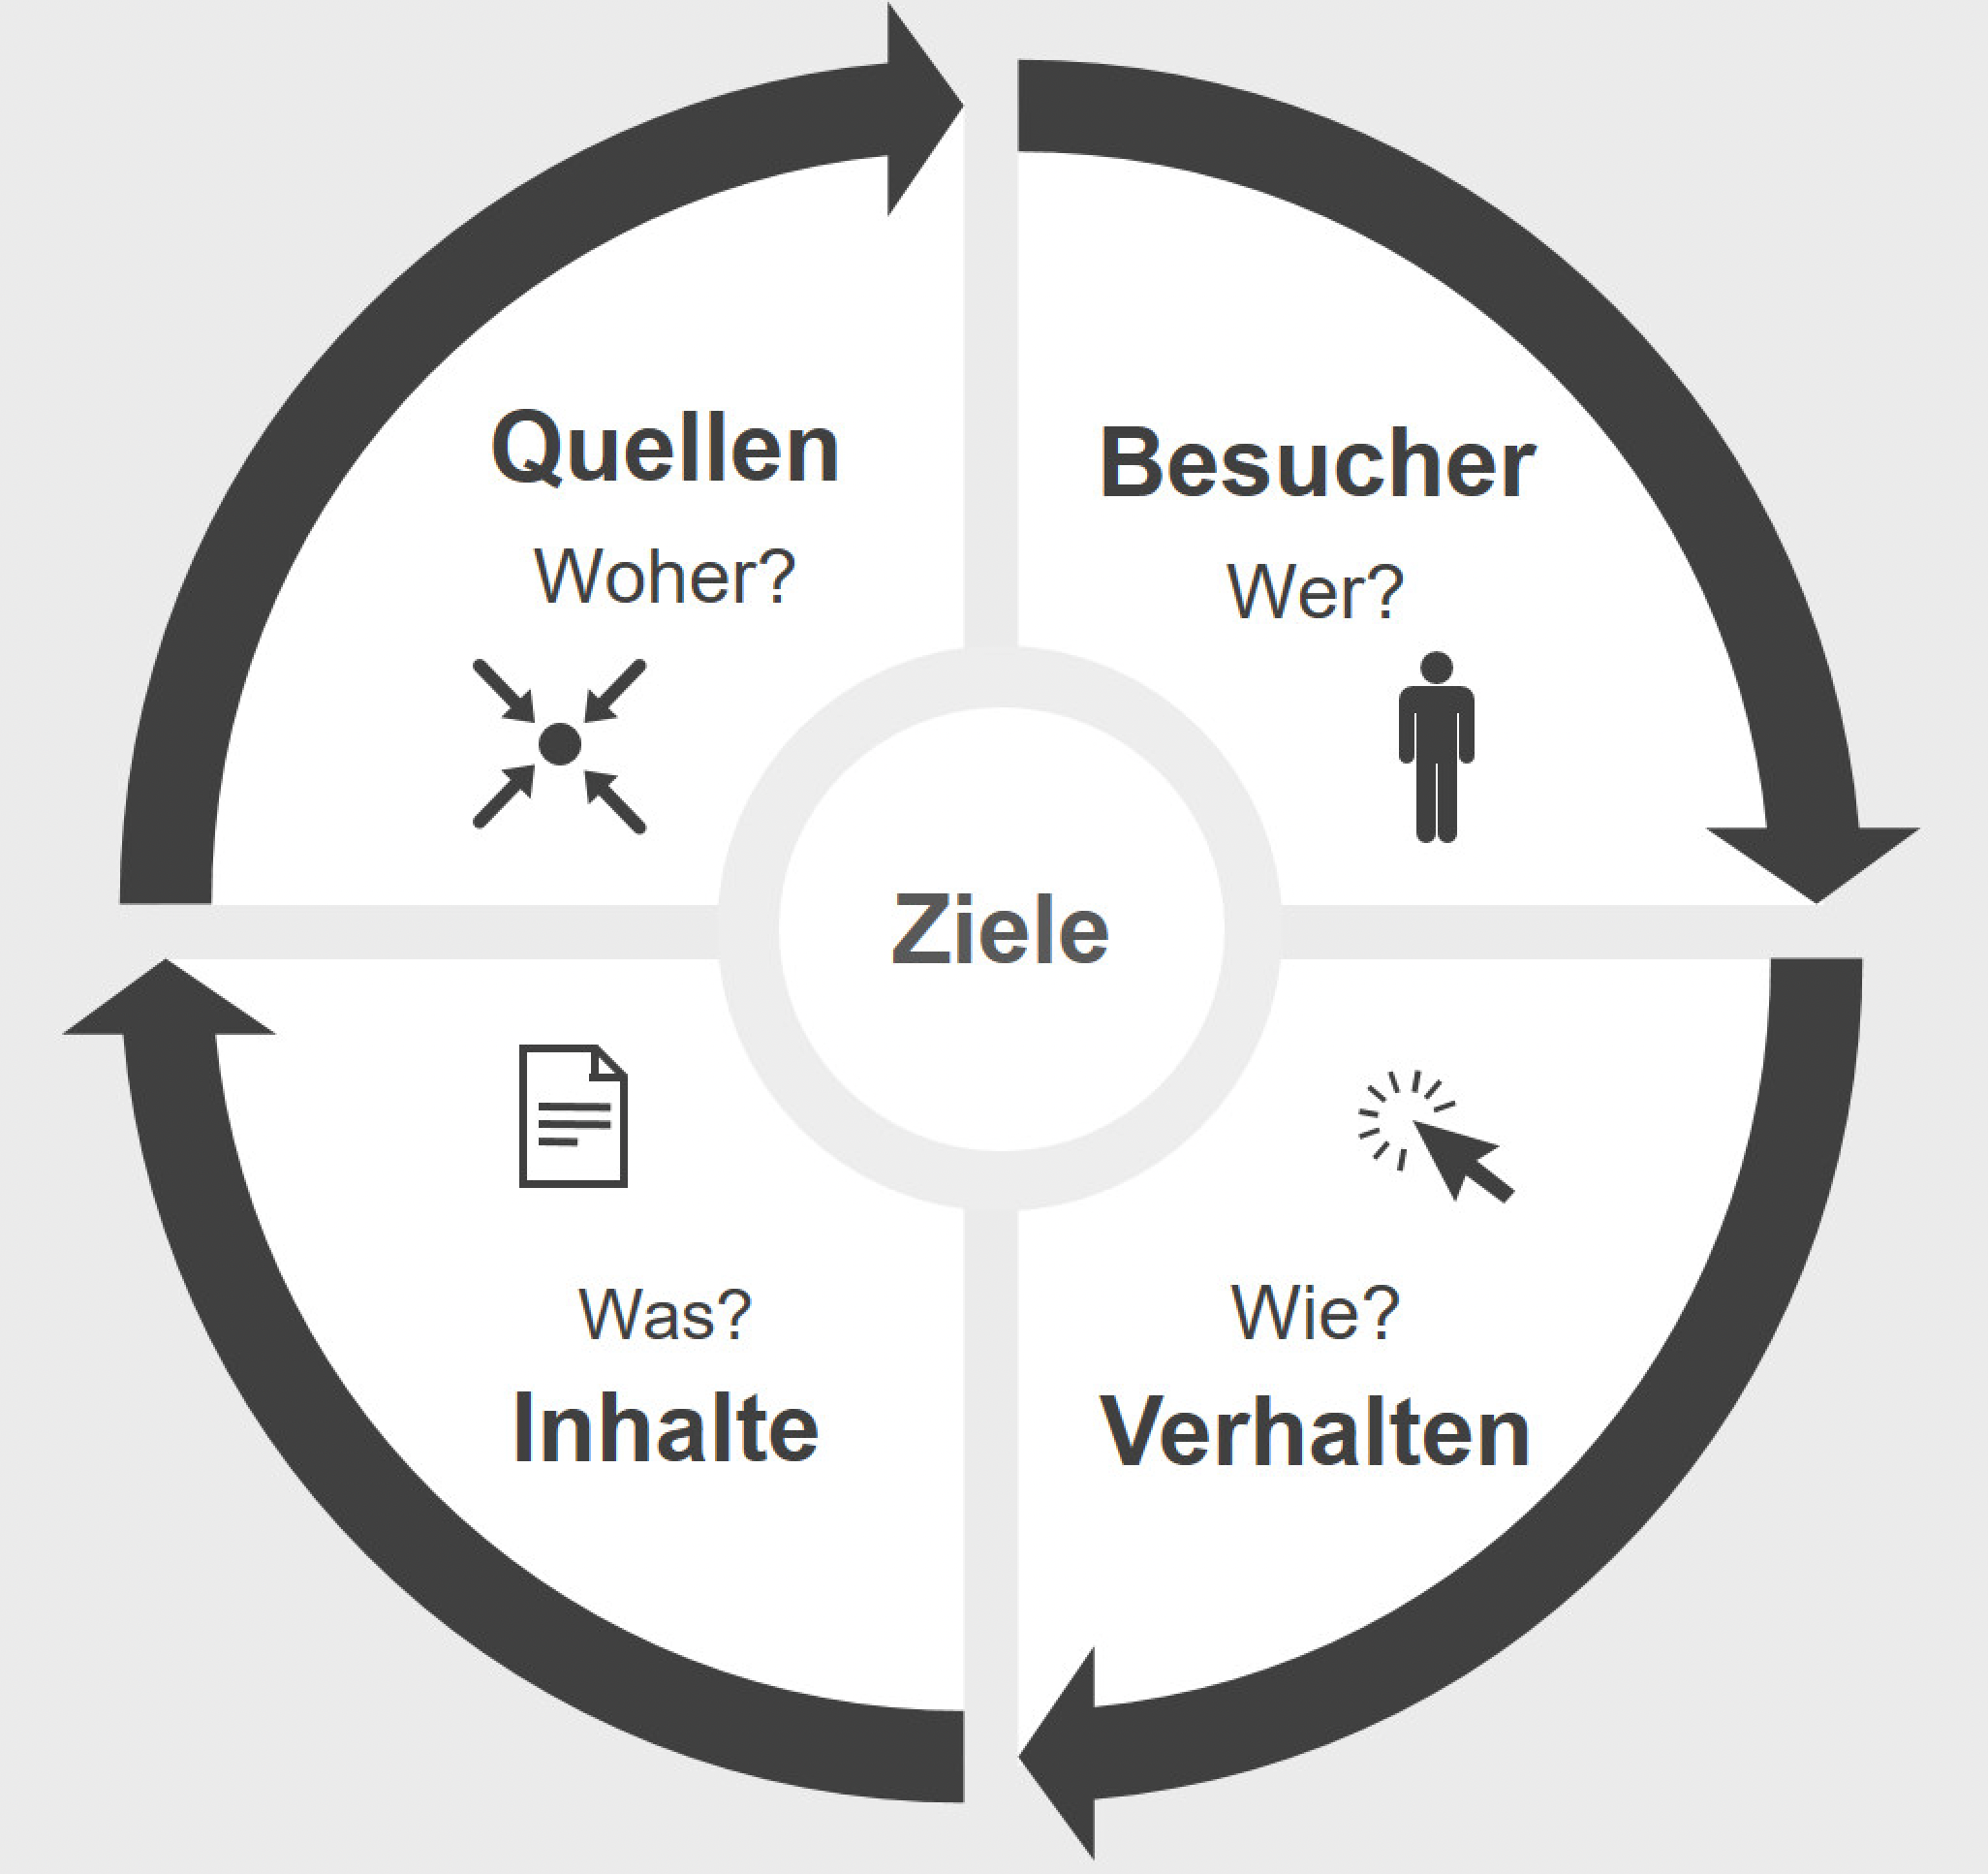
\includegraphics[width=0.5\textwidth]{images/dimensionen.png}%
    \caption{Dimensionen einer Website [Has19]}%
    \label{fig:dimensionen}%
\end{figure}

Durch die Anordnung der Indikatoren in vier Dimensionen – Quellen, Besucher, Inhalte und Verhalten – wird deutlich, dass die Ziele im Zentrum aus der Analyse der Bereiche abgeleitet werden. Die Zuordnung der KPIs zu den entsprechenden Dimensionen ist den Tabelle~\ref{tab:kpi_uebersicht} anahnd der Farbauswahl zu erkennen.

Die KPIs aus Tabelle~\ref{tab:kpi_allgemein} werden dementsprechend auf jeder Dashboardseite in der Dimension Besucher angezeigt.

Auf der Dashboardseite "Übersicht" bezieht sich die Dimension "Quellen" auf externe Traffic-Quellen von welchen ein Besucher auf das Bildungsportal gelangt ist. Hierbei soll die Frage: "Wo kommt denn unser Traffic eigentlich her? [Hassler,2019,Kap.6.2]" beantwortet werden. Auf den anderen Dashboardseiten wird für diese Dimension die interne Navigation zwischen den einzelnen Webseiten betrachtet.

Dimension Inhalte..

Dimension Verhalten...

-> Tabellen einteilen + färben, KPIs besser formulieren, und beschreiben

\section{Visualisierungsmethoden}
%Nachdem die Struktur des Dashboards und die Organisation der %KPIs definiert wurden, stellt sich die Frage, welche %Visualisierungsmethoden am besten geeignet sind, um die %Daten verständlich und aussagekräftig darzustellen.

\section{Grafana als Visualisierungslösung}
Für Vergleich der Datenanbindungsmöglichkeiten: https://alexandre.deverteuil.net/post/visualize-matomo-metrics-in-grafana/

-> außerdem Grafana Labs als Quelle für die Anforderungen und wie diese im Grafana umgesetzt werden können












